
\documentclass[letterpaper, 10 pt, conference]{ieeeconf}  % Comment this line out if you need a4paper

\pdfminorversion=4

\usepackage[english]{babel}
\usepackage{graphicx}
\usepackage{float}
% \usepackage[options ]{algorithm2e} %algorithms
\usepackage[linesnumbered,lined,ruled,vlined]{algorithm2e}
\usepackage{xcolor}
\usepackage{amsmath}
\usepackage{enumitem}
\usepackage{makecell}
\usepackage{multirow}
\usepackage{todonotes}
\newcounter{todocounter}
\newcommand{\shubodh}[1]
{\stepcounter{todocounter}
	\todo[color=green!40,author=Shubodh, inline]{\thetodocounter: #1}
}
\newcommand{\satyajit}[1]
{\stepcounter{todocounter}
	\todo[color=blue!40,author=Satyajit, inline]{\thetodocounter: #1}
}
\newcommand{\tushar}[1]
{\stepcounter{todocounter}
	\todo[color=yellow!40,author=Tushar, inline]{\thetodocounter: #1}
}
\newcommand{\udit}[1]
{\stepcounter{todocounter}
	\todo[color=cyan!40,author=Udit, inline]{\thetodocounter: #1}
}
\newcommand{\ravi}[1]
{\stepcounter{todocounter}
	\todo[color=orange!40,author=Ravi, inline]{\thetodocounter: #1}
}
\newcommand{\mk}[1]
{\stepcounter{todocounter}
	\todo[color=pink!40,author=MK, inline]{\thetodocounter: #1}
}


%\documentclass[a4paper, 10pt, conference]{ieeeconf}      % Use this line for a4 paper

\IEEEoverridecommandlockouts                              % This command is only needed if 
% you want to use the \thanks command

\overrideIEEEmargins                                      % Needed to meet printer requirements.

\title{\LARGE \bf
	Topological Mapping for Manhattan-like Repetitive Environments*
	%\tushar{Topological Mapping for Manhattan-like Environments with repetitive substructures}
}

% 
\author{Sai Shubodh Puligilla$^{*}$, Satyajit Tourani$^{*}$, Tushar Vaidya$^{*}$, Udit Singh Parihar$^{*}$, \\ Ravi Kiran Sarvadevabhatla and K. Madhava Krishna% 
	\thanks{*Denotes authors with equal contribution}% 
	\thanks{This work was supported by Rapyuta Robotics.All authors associated with Robotics Research Center, KCIS, IIIT Hyderabad, India
		{\tt\small \{ravi.kiran,mkrishna\}@iiit.ac.in}}%
}
\begin{document}
	
	
	
	\maketitle
	\thispagestyle{empty}
	\pagestyle{empty}
	
	
	\begin{figure*}[ht]
		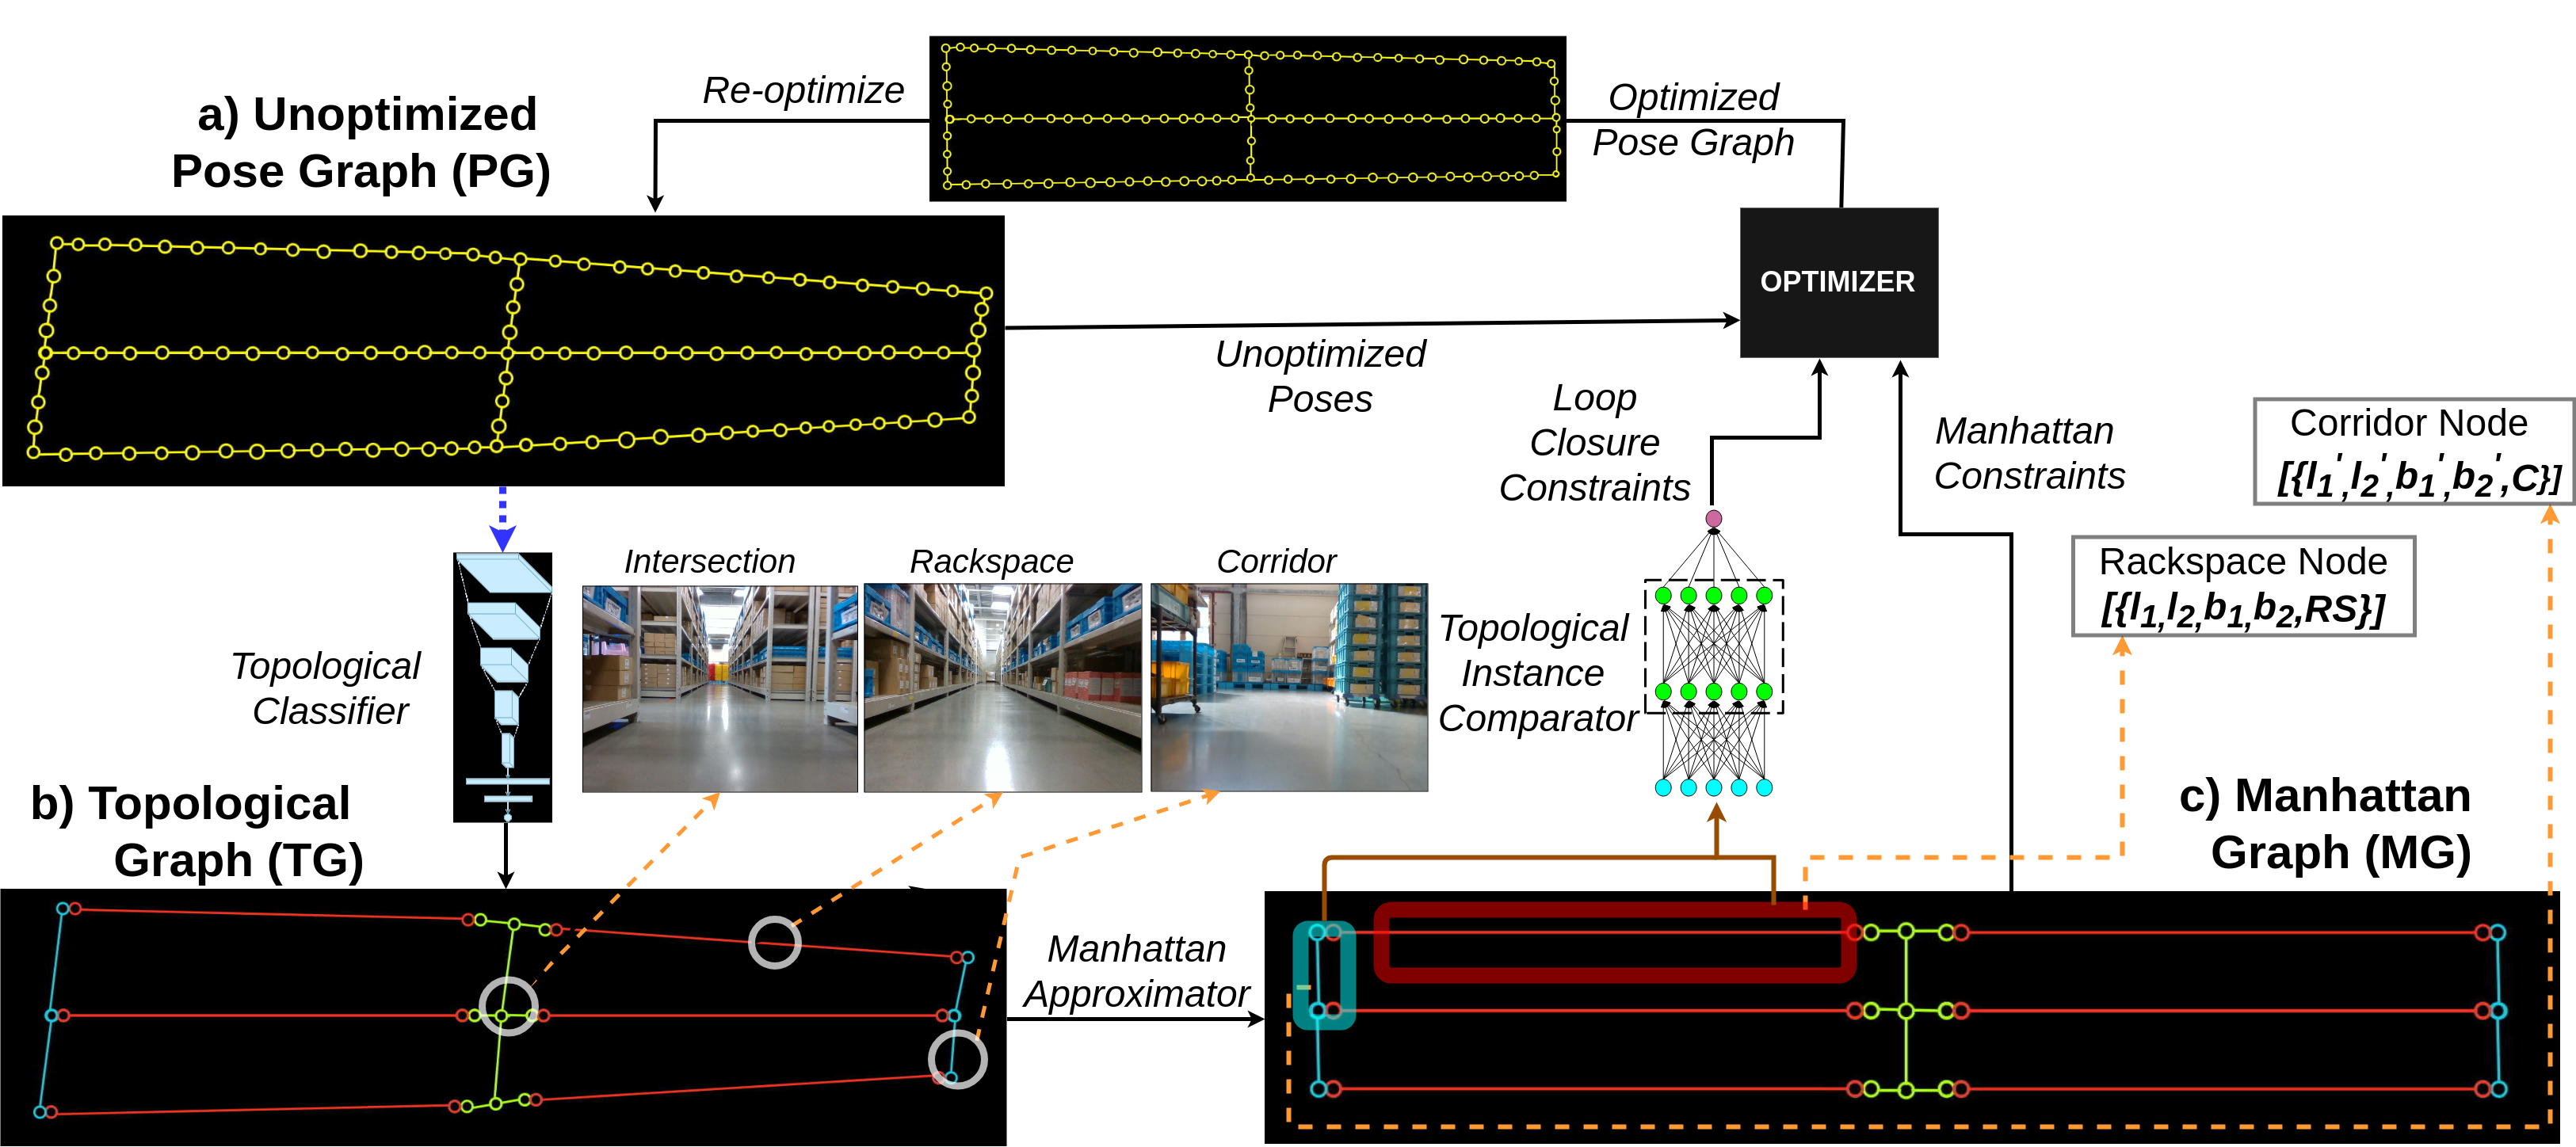
\includegraphics[width=500px]{pic/pipeline_FINAL0434.png}
		\caption{Overall formulation presented with input as Pose-graph and CNN based classifier to classify regions. These classification labels are used to propose potentially similar regions in pose-graph using topological instance comparator which generates more constraints for pose graph. Additionally we generate topologically consistent graph called Manhattan graph which helps add more constraints in pose-graph eventually giving more relevant constraints to pose-graph to increase accuracy. The blue dotted arrow shows the start of the pipeline and then follows a feedback like structure.}
		\label{fig:fig1_pipeline}
	\end{figure*}
	%%%%%%%%%%%%%%%%%%%%%%%%%%%%%%%%%%%%%%%%%%%%%%%%%%%%%%%%%%%%%%%%%%%%%%%%%%%%%%%%
	\begin{abstract}
		We showcase a topological mapping framework for a challenging indoor warehouse setting. At the most abstract level, the warehouse is represented as a Topological Graph where the nodes of the graph represent a particular warehouse topological construct (e.g. rackspace, corridor) and the edges denote the existence of a path between two neighbouring nodes or topologies. At the intermediate level, the map is represented as a Manhattan Graph where the nodes and edges are characterized by Manhattan properties and as a Pose Graph at the lower-most level of detail. The topological constructs are learned via a Deep Convolutional Network while the relational properties between topological instances are learnt via a Siamese-style Neural Network. In the paper, we show that maintaining abstractions such as Topological Graph and Manhattan Graph help in recovering an accurate Pose Graph starting from a highly erroneous and unoptimized Pose Graph. We show how this is achieved by embedding topological and Manhattan relations as well as Manhattan Graph aided loop closure relations as constraints in the backend Pose Graph optimization framework. The recovery of near ground-truth Pose Graph on real-world indoor warehouse scenes vindicate the efficacy of the proposed framework.
	\end{abstract}
	% post backend SLAM optimization
	
	%%%%%%%%%%%%%%%%%%%%%%%%%%%%%%%%%%%%%%%%%%%%%%%%%%%%%%%%%%%%%%%%%%%%%%%%%%%%%%%%
	% \vspace*{240px}
	\section{Introduction}
	
	This paper explores the role of topological understanding and the concomitant benefits of such an understanding to the SLAM framework. Figure-\ref{fig:fig1_pipeline}a shows an erroneous Pose Graph (PG) while Figure-\ref{fig:fig1_pipeline}b shows topology-level nodes of the Pose Graph and the topological-label-encoded edges. A Deep Convolutional Network infers the topological label corresponding to every pose. The PG is transformed into a Manhattan Graph (MG) (Figure-\ref{fig:fig1_pipeline}c) where Manhattan-like relations exist between adjacent nodes. While the MG facilitate seamless loop detection between a pair of Manhattan nodes, such relations when integrated with a back-end SLAM framework, enables recovery of an optimized pose-graph and corresponding map. The colours of the map represent the corresponding topologies perceived by the robot at those nodes. The crux of the paper lies in detailing the framework and its efficacy in challenging real warehouse settings and as well as in realistic simulator frameworks such as Gibson~\cite{xiazamirhe2018gibsonenv}.
	
	There have been a number of works in this area and a detailed review of such methods can be seen in \cite{garcia2015vision}. Prominent and well cited amongst these include \cite{ulrich2000appearance, sunderhauf2012switchable, pronobis2006discriminative, ranganathan2006rao,kosecka2003qualitative }. Most of these methods are focused exclusively on vision based loop detection with invariant descriptors. Many relate to an individual image as a distinct topology of the scene without relating such nodes to a meta-level label such as a rackspace, corridor, intersection etc. Some seminal works as \cite{agarwal2013robust} show recovery from wrong loop closures in a Manhattan environment though they don't discuss how the original MG is constructed and how such relations can be integrated into a backend SLAM. \cite{ranganathan2006bayesian} show how a Bayesian inference over topologies can be performed to obtain more accurate topological maps. However, the topological constructs are at a local image level than at a larger meta-level such as in this paper. In other words, \cite{ranganathan2006bayesian} does not entertain  notions of meta-level topological labels that go beyond an immediate lower-level topology restricted to the scene seen by the robot.
	
	In this paper, we distinguish ourselves by portraying how higher level/meta level topological constructs that go beyond an immediate frame/scene and the relations that they enjoy amongst them percolate to a lower level pose-graph and elevate their metric relations. In fact, we recover close to ground truth floor plans from a highly disorganized map at the start. This is the essential contribution of the paper. In addition, the following constitute our contributions:
	\begin{enumerate}
		\item A deep network architecture capable of learning warehouse topologies and ablation studies over the same.
		\item A Multi-Layer Perceptron (MLP) classifier which resolves topological element ambiguity and helps achieve an accurate topological graph purely based on Manhattan relations. Ablation studies are performed to signify the effectiveness of the classifier. 
		\item We showcase a backend SLAM framework that integrates loop closure relations from an intermediate level Manhattan Graph to the lowest level Pose Graph and elevate a disoriented unoptimized map to a structured optimized map which closely resembles the floor plan of the warehouse. Apart from the loop closure relations, the SLAM integrates other Manhattan relations to the pose graph. Ablation studies show the utility of both loop and Manhattan constraints as well as the superior performance of an incremental topological SLAM over a full batch topological SLAM.
		\item We also show how the two-way exchange between the $MG$ and $PG$ further improves the accuracy of the $PG$. 
		% \mk{This seems too low-level here. Could be moved to discussion or conclusion -- In other words not only does the constraints induced by the $MG$ on $PG$ improve $PG$’s accuracy but also that an improved $PG$ feeds back to the $MG$ and prevents $M$ from diverging. An improved $MG$ in turn induces more accurate constraints on $PG$ resulting in better accuracy. }
		This two-way exchange between between the various levels of representation is unique to this effort.  
	\end{enumerate}
	
	
	\section{Methodology}
	Consider an unoptimized pose graph $PG$ represented by its nodes as $V_{p}$ and edges as $E_{pg}$. The edges relation are of the following kinds:
	\begin{itemize}
		\item Odometry relation between successive nodes.
		\item Loop closure relation between a pair of nodes.
		\item Manhattan relation between a pair of nodes.
	\end{itemize} 
	
	We obtain odometry relations from fused ICP and wheel odometry estimates which gives us the initial pose graph which is highly erroneous. We then leverage the topological and Manhattan level awareness to generate the loop closure and Manhattan relations and use them for pose graph optimization to recover accurate graphs. This whole process is divided into 3 sub-sections:
	
	\begin{enumerate}
		\item Topological categorization using a convolutional neural network classifier and its graph construction.
		\item Constructing Manhattan Graph from the obtained Topological Graph and predicting loop closure constraints using Multi-Layer Perceptron.
		\item Pose graph optimization using obtained Manhattan and loop closure constraints.
	\end{enumerate}
	
	Each part of the pipeline is described in each sub-section below, followed by experiments and results which are explained in the next section.
	
	\subsection{Topological Categorization and Graph Construction}
	\label{sec:semantic_place_cat}
	
	
	Every node $V_{i} \in V_{pg} $ is associated with a topological label $L(V_{i})$ for $L_{i} \in L=\{rackspace, corridor, transitions\}$ for a warehouse scene. To obtain these topological labels from visual data, we train a Convolutional Neural Network (CNN) configured for classification. The training data consists of RGB images resized to $224 \times 224$ and paired with topological node labels. For our warehouse setting, the labels are \texttt{Rackspace, Corridor, Intersection}:
	\begin{itemize}
		\item \texttt{Rackspace}: Location on path between two rackspaces
		\item \texttt{Corridor}: Location on the warehouse boundary path common to rackspaces
		\item \texttt{Intersection:} A transition location on the path 
	\end{itemize} 
	
	Figure-\ref{fig:fig1_pipeline} entails examples of frames and their topological labels. We train a ResNet-18~\cite{he2016deep} architecture pre-trained on ImageNet~\cite{imagenet_cvpr09} with its final layer replaced by a $3$-neuron fully connected layer, corresponding to the possible topological node labels. During training, we optimize the network to minimize cross-entropy loss. To account for class imbalance, we use class-weighted loss~\cite{johnson2019survey} with the following set of weights: \texttt{Rackspace}$:2.48$, \texttt{Corridor}$:2.16$, \texttt{Intersection}$:7.38$. The CNN is fine-tuned for $356$ epochs using Adam optimizer with a learning rate of $0.001$ for the pre-trained ResNet-18 layers and a learning rate of $0.005$ for the final layer weights. We stop training when the validation loss starts to increase. For training, we use $33{,}273$ images from two warehouses with a mini-batch size of $8$. To evaluate the trained network, we use $21{,}200$ images. The results are presented in the next section.
	
	After obtaining the inferred labels from the CNN, we group together the adjacent nodes that share the same label. Thus, a node in Topological Graph $TG$ consists of two positions from the dense Pose Graph $PG$, i.e.  the starting and ending positions of that topology.  
	
	\begin{figure*}
		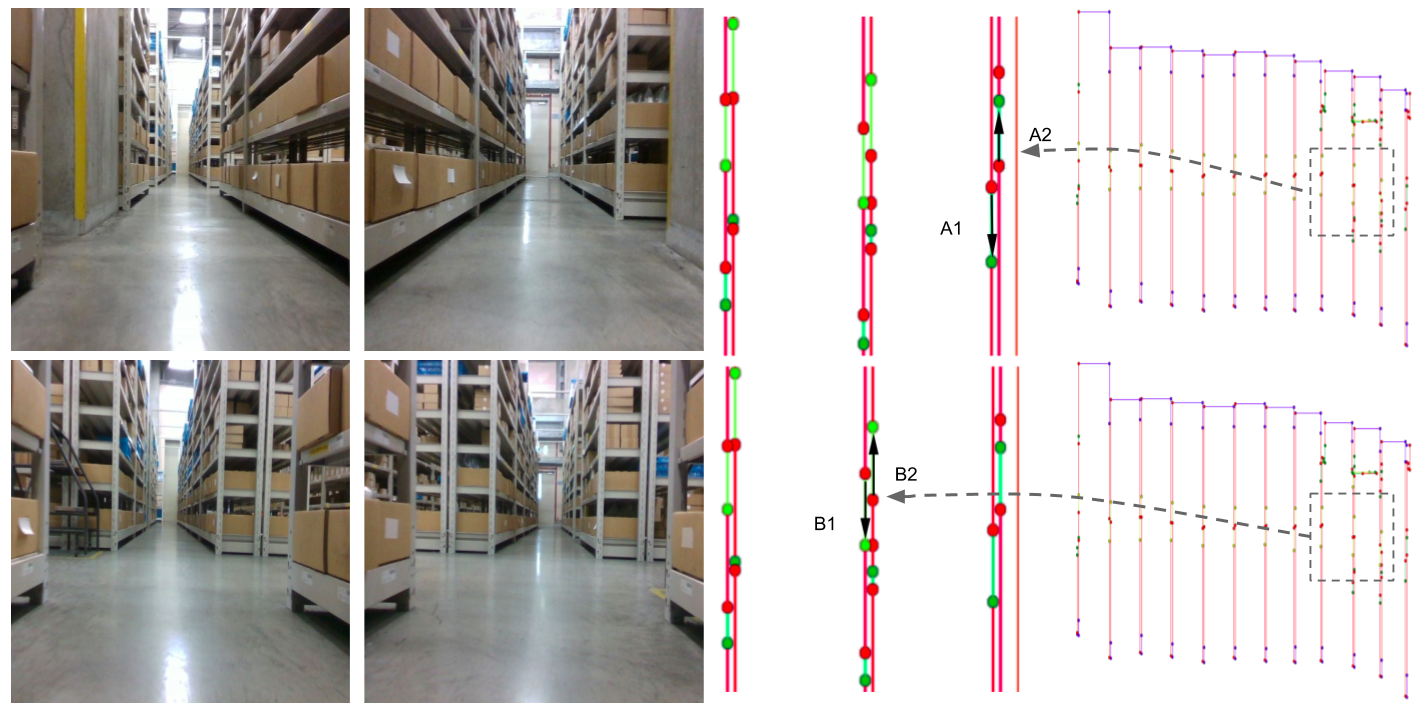
\includegraphics[width=480px, height=6cm]{pic/diff_images_flipped.png}
		\caption{We demonstrate the detection of similar nodes using MLP. Along each row we show image pairs along with its manhattan trajectory map and the location of both image pairs on the manhattan map. The gray dotted box indicate the location of the overlapping intersection nodes which belong to the same topology in the global manhattan map. The gray dotted arrow points to the overlapping intersection nodes shown zoomed-in. The black arrows in the opposite direction depict the same region but viewed from opposite directions by the robot. The top row shows the location of a particular 3-way intersection region from opposite views which belong to the same topology. The bottom row shows the location of a particular 4-way intersection region from opposite views which belong to the same topology. We denote the forward viewpoint of the 3-way intersection by A1. A2 denotes the same intersection from a backward viewpoint. B1 denotes the forward viewpoint of the 4-way intersection. B2 denotes the same 4-way interction from the opposite backward viewpoint. We demonstrate detection of similar nodes which belong to the same topology at opposite viewpoints which is known to be a difficult task.}
		\label{fig:boat22}
	\end{figure*} 
	\subsection{Manhattan Graph Construction and Constraint Prediction using MLP}
	\label{manhatten_construction}
	We now explain how the Topological Graph TG of the last section is converted to a Manhattan Graph, MG. We denote each note in the $MG$ as a meta-node, $M_{j} \in MG$, where $M_{j}$ corresponds to a collection $C$ i.e. $V_{i}, V_{i+1},.., V_{i+n}$ of $PG$ nodes, such that we write $V_{i} \in C(M_{j})$ and $L(M_{j}) = L(V_{i}) $ for every $PG$ node in the collection set $C$. A new meta-node is formed when there is a change in the label.
	
	The pose graph nodes, their corresponding topology labels shown in the color denoting the label, the collection of such nodes that constitute a meta node also shown in the same color in the $MG$ are portrayed in figure~\ref{fig:Posegraph Optimization pipeline}	
	The MG relies on two essential measurements for its construction. 
	\begin{itemize}
		\item The length $l$ of traversal or the length of topologies such as corridor or a rackspace.
		\item The angle $\phi$ made between two corridors/two rackspaces/rackspace and corridor via an intersection. 
	\end{itemize} 
	
	The length of the traversal is obtained by integrating fused odometry and ICP based transformations between two successive nodes of the Pose Graph that belong to the same meta node in the Manhattan Graph. The angle made as the robot moves from one topology (rackspace/corridor) to another (rackspace/corridor) via an intersection is estimated by fusing odometry and scan matching ICP measurements and integrating them over the traversal through the Intersection. This angle is binned to the closest multiple of $\pi/2$ as one of $\frac{-\pi}{2}, 0, \frac{\pi}{2}, \pi$. We use these sets of obtained lengths $l$ and angles $\phi$ along with the category of the meta node $M_{j}$ i.e. $L(M_{j})$ as attributes as input to a Siamese-style MLP neural network in order to determine if any two nodes in $MG$ are the same instance of a topological construct. In other words, the MLP determines if any two nodes in $MG$ correspond to the same topological area of the workspace. 
	
	The training data for the MLP consists of what we have described as ``meta-nodes" above. Each meta-node is a tuple consisting of $\{X_{start}, Y_{start}, X_{end}, Y_{end}\}$. The four values of the tuple denote the starting and ending displacement co-ordinate of a particular node with respect to a global origin (global origin is the point from where the robot starts moving in the warehouse). $X_{start}$ and $X_{end}$ denote the displacement co-ordinates in the x-direction. $Y_{start}$ and $Y_{end}$ denote the displacement co-ordinates in the y-direction. We create training data on the fly since we know the general structure of our warehouse and hence can create nodes synthetically using random numbers with similar lengths. The architecture is a Siamese network \cite{bromley1994signature} which consists of two hidden layers as shown in Figure-\ref{fig:MLP_fig}. We apply contrastive loss on the output obtained from the Siamese network to constrain semantically similar ``meta-node" representations to lie closer to each other. During inference, the MLP compares two nodes of the Manhattan Graph and predicts if the nodes correspond to the same topological instance. We base our approach on two strong assumptions:
	\begin{itemize}
		\item Each node comprises of one contiguous region of one particular category.
		\item Each node has displacement only in one direction. (Along x or y). 
	\end{itemize}
	\begin{figure}
		\centering
		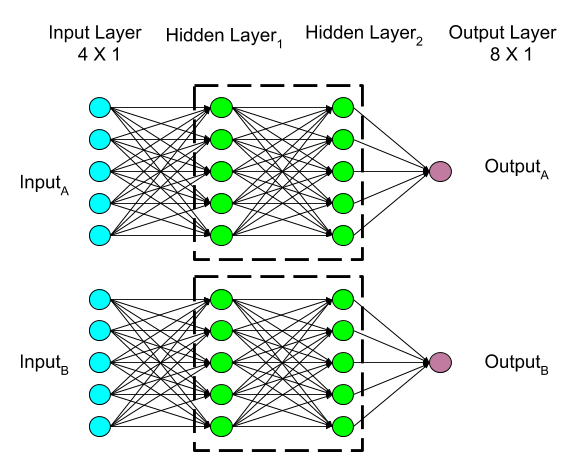
\includegraphics[width=\linewidth, height=6cm]{pic/mlp_architecture.png}
		\caption{Architecture of the Multilayer Perceptron. The architecture is a siamese like network where we pass the $4 \times 1$ input to the 2-layered MLP and we get an $8 \times 1$ output for each node. We do this for both nodes to be compared and then perform a contrastive loss on both the outputs so as to condition the output vectors based on whether the node-pair's ground truth label is same(S) or different(D). The dotted boxes denote sharing of the network weights.}
		\label{fig:MLP_fig}
		
	\end{figure}
	
	The classification that results from the MLP is particularly powerful due to its ability to classify two topological instance to be the same even when viewed from opposing viewpoints. This is shown in Figure-\ref{fig:boat22} where the same topology is viewed from opposite viewpoint and have little in common. Yet the MLP's accurate classification of them to be the same instance becomes particularly useful for the Pose Graph optimization described in the next section. 
	
	The MLP's non reliance on perceptual inputs also comes in handy for repetitive topologies. Warehouse scenes are often characterizes by repetitive structure and are prone to perceptual aliasing. The classification accuracy of the MLP is unaffected by such repetitiveness in the environment since it bypasses perceptual inputs. Yet the MLP does make use of perceptual inputs minimally in that it attempts to answer if the two nodes in the MG are the same instances only if the topological labels of the two nodes are predicted to be the same by the CNN.
	
	\subsection{Pose Graph Optimization}
	
	%The classification of two instances, $M_{i}, M_{j}$ to be the same by the MLP is made use of by the Pose graph optimizer in the following manner.
	
	The Manhattan relation that exists between two nodes $M_{i},M_{j}$ and represented as $ R(M_{i},M_{j}) = <\Delta x_{ij}, \Delta y_{ij}, \Delta\theta_{ij}>$ serves as a Manhattan constraint between the nodes corresponding to $M_{i},M_{j}$ in the pose graph (in a manner consistent with the edge relations given in posegraph libraries such as G2O \cite{kummerle2011_g2o}, GT-SAM \cite{kaess2008isam}). $\Delta\theta_{ij}$ is typically $0^\circ$ or $180^\circ$ depending on whether the topology is being revisited with the same or opposing orientation.
	
	The output of the MLP classifier is also used to invoke loop closure constraints. A pair of nodes classified to be the same topological construct by MLP corresponds to two sets of pose-graph nodes in the unoptimized graph belonging to the same area. Multiple loop closure relation are thus obtained between the pose-graph nodes of these two sets. Apart from these, there exist immediate Manhattan relations between two adjacent rackspaces or two adjacent corridors or a rackspace adjacent to a corridor mediated through an intersection. All such relations that exist in the Manhattan Graph as well as the loop closure relations percolate to the nodes in the PG as described further below.
	
	In effect the optimizer solves for \cite{sunderhauf2011brief}:
	%\textit{Equation 1}
	
	\begin{align*}
	X^{*} &= \underset{X}{argmax}\medspace P(X|U) \\
	&= \underset{X}{argmax}\medspace \prod_{i}P(x_{i+1} | x_{i}, u_{i}) \underset{\textit{Loop Closure Constraints}}{\underbrace{\prod_{i \in C(M_{i}), j \in C(M_{j})}P(x_{j} | x_{i}, c_{ij})}}\\ &{\underset{\textit{Manhattan Constraints}}{\underbrace{\prod_{i \in N(M_{i}), j \in N(M_{j})}P(x_{j} | x_{i}, m_{ij})}}} 
	\end{align*}
	
	where $P(X|U)$ is estimation's probability of posegraph $X$ over set of constraints $U$, $x_{i}$ and $u_{i}$ are $i^{th}$ pose and controls of the robot. The loop closure relation $c_{ij}$ between nodes $i$ and $j$ is obtained using ICP. There are in principle $n(C(M_{i})) * n(C(M_{j}))$ loop closure relations that are possible between topological constructs $M_{i}, M_{j}$ where $C(M_{i})$ is the collection set of Manhattan node $M_{i}$ as described before  and $n(P)$ is the cardinality of the set $P$. Whereas in practice we only sample a subset of such relations to constrain the graph.
	
	Similarly, the graph is also constrained by Manhattan relations $m_{ij}$ that are invoked between the pose-graph nodes that constitute the sets $N(M_{i})$ and $N(M_{j})$ where $N(M_{i})$ and $N(M_{j})$ represent pose graph nodes of the topological construct area $M_{i}$. 
	
	Typically $N(M_{j}) \subseteq C(M_{j})$. More formally, let $S$ be the set that enumerates all loop closure pairs discovered by the MLP over a Manhattan Graph MG. i.e $S = \{(M_{i},M_{j}), (M_{j},M_{k}), ..., (M_{p},M_{q})\} $, where each element of the set is a loop closure pair on the graph and $\{M_{i},M_{j},..,M_{q}\}$ are the nodes of the $MG$. Let $i$ be an iterator iterating over the element of $S$, $S(i) = (M_{p}, M_{q})$.  Let $LC$ be the set of all loop closure relation, $C_{ij}$ obtained for every $S(i) \in S$ by sampling from the $n(C(M_{i})) * n(C(M_{j}))$ number of loop closures possible for every $S(i) \in S$. Similarly, let $M$ be the set of all Manhattan relation $m_{ij}$ obtained for every $S(i) \in S$ from the neighbouring nodes in the unoptimized graph $N(M_{i}), N(M_{j})$ for every $S(i) = (M_{i},M_{j}) \in S$. Then
	
	%\textit{Equation 2}
	
	\begin{align*}
	X^{*} &= \underset{X}{argmax}\medspace \prod_{i}P(x_{i+1} | x_{i}, u_{i}) 
	\prod_{c_{ij} \in LC}P(x_{j} | x_{i}, c_{ij}) \\
	&{\prod_{m_{ij} \in M}P(x_{j} | x_{i}, m_{ij})}
	\end{align*}
	
	
	%\subsection{Algorithm for posegraph optimization}
	\begin{algorithm}[h!]
		\SetAlgoVlined
		
		\KwResult{optimized pose-graph using topological information}
		\KwData{$PG=\{V_{pg},E_{pg}\}$,MG = \{$v$,$e$ \mid $v \subseteq V_{pg}, e \subseteq E_{pg}$\}}
		propose MG using algorithm described in \ref{manhatten_construction}\\
		propose pairs of loop closure estimates using topological instance comparator\;
		
		\While{Not All nodes are optimised}{
			propose pairs of loop closure estimates using topological instance generator\; \\ 
			generate ICP estimates for proposed pairs\; \\
			search points based on Manhattan graphs around proposed pairs which follows Manhattan constraints\; \\
			add into the pose-graph as additional constraints\; \\
			Optimize pose-graph\; \\
			regenerate Manhattan graph based on optimized pose-graph\;
			repeat step 3.\;
		}
		\caption{Strategy for optimizing pose-graph with Manhattan and topological constraints.}
	\end{algorithm}
	
	
	\section{Experimentation and Results}
	\subsection{Topological Categorization in a Real Warehouse Setting}
	
	\begin{figure}[!htbp]
		% \centering
		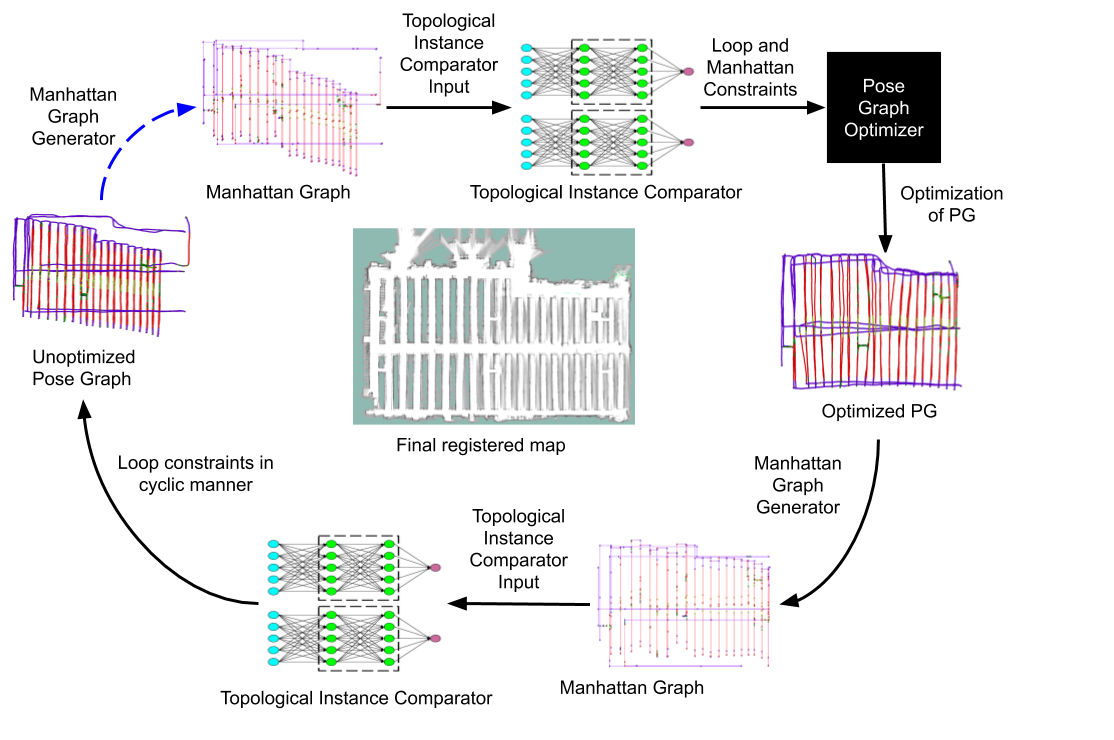
\includegraphics[width=8.8cm,height=6cm]{pic/algorithm_optimization.png}
		\caption{We start with the unoptimized Pose Graph with drift (shown by dotted-blue arrow) and obtain its Manhattan Graph. The nodes of the Manhattan graph are then passed to the Topological Instance Comparator which acts like a Topological Instance comparator and gives out node pairs which belong to the same topology. This is then passed to the Pose Graph Optimizer which gives us optimized Pose Graph. We then obtain the Manhattan graph of the optimized Pose Graph. The nodes of this graph are passed to the Topological Instance comparator which gives us improved(more accurate) loop pairs. This complete pipeline is done multiple times in a cyclic manner till convergence. We finally get a registered map which is shown in the center.}
		\label{fig:Posegraph Optimization pipeline}
	\end{figure}
	
	The performance of the topological node classification CNN (Section \ref{sec:semantic_place_cat}) with comparison to the baseline frontier detection can be viewed in Table \ref{CNN_accuracy_conf_results}. For the combined dataset, the network is able to classify the rackspace and corridor with very low false positives and false negatives with precision and recall more than $94 \%$ each. However, it is relatively difficult to classify the third class i.e. intersection as there is not much semantic consistency as the robot moves from one topology to another, which is reflected in the fact that the recall value is quite low, about $78 \% $. We explain how this inaccuracy affects the downstream modules in the Section \ref{sec:robust_analysis}.
	
	
	\begin{table}[h]
		\caption{CNN Classification Results.}
		\label{CNN_accuracy_conf_results}
		\begin{center}
			\begin{tabular}{|c||c||c||c|}
				\hline
				\textbf{\thead{Warehouse \\ dataset}} & \textbf{Accuracy} \\
				\hline
				1\&2 &93.75\\
				\hline
				1&95.15\\
				\hline
				2&89.06\\
				\hline
			\end{tabular}
			\quad
			\begin{tabular}{|c||c||c|}
				\hline
				\multicolumn{3}{|c|}{\textbf{\thead{Metrics for Combined Data (1\&2)}}} \\
				\hline
				\textbf{\thead{Category}} & \textbf{Precision} & \textbf{Recall} \\
				\hline
				Rackspace & 94.2 & 96.3 \\
				\hline
				Corridor & 96.3 & 96.4 \\
				\hline
				Intersection & 85.6 & 78.1 \\
				\hline
			\end{tabular}
		\end{center}
	\end{table}
	
	
	\subsection{Efficacy of Loop Closure Constraint Prediction using MLP}
	\begin{itemize}
		\begin{table}[h]
			\caption{MLP Results. }
			\label{CNN_results_accuracy}
			\begin{center}
				\begin{tabular}{|c||c||c||c|}
					\hline
					\textbf{Network Type} & \textbf{Warehouse-1} &  \textbf{Warehouse-2}\\
					\hline
					MLP & 71.2 & 67.7\\
					
					\hline
				\end{tabular}
			\end{center}
		\end{table}
	\end{itemize}
	
	We showcase our pipeline on two different warehouses. There were two experiments performed. First, we  sample our training data according to the layout and length constraints of warehouse-1 and use the data-points of warehouse-1 as the lone testing data. In our second experiment, we train our MLP specifically according to the layout and length constraints of warehouse-2. 
	
	The detection of nodes belonging to the same topology was observed to be accurate at the initial phase of the trajectory. The latter part of the trajectory was not accurate and had drift due to which the detection of node-pairs was observed to be inaccurate(Unoptimized Pose Graph shown in  Figure-\ref{fig:Posegraph Optimization pipeline}) . We were able to improve the accuracy of the MLP and were able to generate accurate loop pairs by performing optimization on the Pose Graph in a cyclic fashion as shown in Figure-\ref{fig:Posegraph Optimization pipeline}
	
	We performed the experiments on both warehouses. The accuracy is calculated by checking for the percentage of the true node pairs. An accuracy of $71.2 \%$ and $67.7 \%$ was observed for the first and the second warehouse respectively. 
	
	\subsection{Pose graph optimization Results}
	
	The ablation study on the type of constraints have been done five stages. The robustness of map recovery increases with each stage which reflects in Absolute Trajectory Error in Table \ref{tab: ate_comparison}. 
	
	\subsubsection{Stages of Map Recovery}
	\begin{enumerate}[label=(\roman*]
		\item \textit{Manhattan constraints: } Only manhattan constraints are used to optimize pose graph, PG. Constraints are extracted from manhattan graph, MG, between nodes proposed by MLP to be similar. 
		\item \textit{Loop Closure and Manhattan constraints: } Apart from Manhattan constraints, Loop Closure constraints as explained in section II-C are also used to constrain the PG. 
		\item \textit{Dense Proposals from MLP: } We consider nodes that have been classified to belong to the same instance with low confidence along with those classified to be the same with high confidence. This increases the number of constraints improving the optimization performance. The wrongly detected loops are filtered based on the loop closure (ICP) residual cost and do not make it to the optimization.
		\item \textit{Dense Proposals by MLP in Feedback Loop: } A feedback loop is invoked on the optimized PG from previous stage. A new MG is computed on the optimized PG, this manhattan graph, MG, is feeded to MLP and sets of constraints are generated in a cyclic manner. This feedback mechanism leads to MLP performance improvement as shown in Table VI and also helps in achieving very low Absolute Trajectory Error, ATE of 1.82 meters on four different maps from 11.57 meters in unoptimized map.
		\item \textit{Incremental formulation: } Performing the feedback strategy from the previous stage in an incremental formulation in ISAM \cite{kaess2008isam} helps us to achieve the lowest ATE of 1.45 meters in our system. This confirms the robustness of our system to recover from highly unoptimized trajectories.
	\end{enumerate}
	
	\subsubsection{Qualitative Results}
	
	We evaluate our system in two challenging real warehouse settings. The warehouse dimensions are $30m \times 50m$ and contains $21$ rackspaces with intermediate corridors and intersections. All experiments  start with highly deformed trajectories. In all the cases, we were able to recover trajectories close to the groundtruth. Note that in our case, the ground-truth trajectory is the optimized map from the cartographer that has been confirmed with warehouse floor plan by our collaborators . These results are shown in Figure 6. The top row shows highly distorted pose graph trajectories while the middle row showcases the results of our optimization framework. The last row depicts the ground truth trajectories. The overall pipeline gets best illustrated with Figure 4.
	
	\subsection{Robustness Analysis}
	\label{sec:robust_analysis}
	
	We analyze the performance of the topological SLAM due to errors in topological classfication due to the CNN and due to failure to detect loops by the MLP. Errors in topology classification manifest as loop detection in the MG. Therefore, the analysis is one of the robustness due to wrong loop detection  wherein both false positive and false negative cases are considered. The robustness to the pose graph optimization stems due from the following features:
	
	\begin{enumerate}
		\item Residuals in the ICP estimated loop closure end up serving as priors to the element of dynamically scaled covariance matrix \cite{agarwal2013robust}, which serves as a robust kernel providing for backend topology recovery even when the number of wrong loop closures increase.
		\item An optimized PG feeds back to the MG and alleviates its error. The improved MG improve the loop detection performance of MLP, which percolate to the PG nodes and further improve its accuracy. Overtime this iterative exchange of information between the various representations improves the robustness of the PG backend.
	\end{enumerate}
	
	\begin{figure}[H]
		\centering
		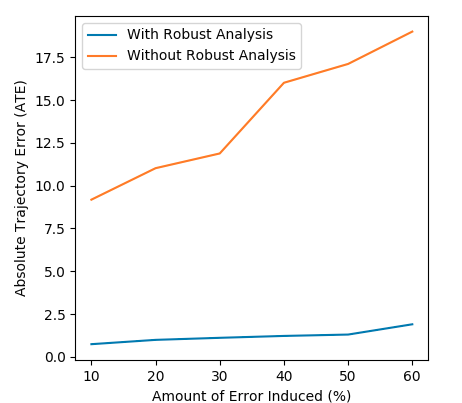
\includegraphics[width=7cm,height=5cm]{pic/robust_analysis_v3.png}
		\caption{Effect of Robust pose-graph optimization with DCS}
		\label{fig:failure_analysis}
	\end{figure}
	To analyse the performance of our robust kernel exclusively in presence of the outliers, we synthetically introduced false positive and false negative loop closure pairs in the constraints for PG. In plot \ref{sec:robust_analysis} X-axis represents \% of loop closure pairs in the data-set having equal amout of false positive and false negative pairs.Y-axis represents Absolute Trajectory Estimates of TG with respect to the ground truth. The Figure \ref{sec:robust_analysis} depicts the performance of our framework due to errors occurred in topology classification and loop detection. 
	
	
	From the analysis of results in plot \ref{sec:robust_analysis} it is evident that gradual increase in outliers can be tolerated by Robust kernel with DCS \cite{agarwal2013robust} as compared with non robust optimization techniques.
	
	
	\begin{table}[ht] %Tushar Editing ....
		\caption{Absolute Trajectory Error(ATE) and Relative Pose Error (RPE) \cite{sturm2012benchmark} for various pose-graphs with respect to ground-truth trajectories}
		\centering
		% 		\renewcommand{\arraystretch}{1.2}
		\begin{tabular}{|p{2.5cm}|c|c|c|c|c|}
			\hline
			\multirow{2}{2.5cm}{\textbf{Method Type}} & 
			\multicolumn{1}{c|}{\textbf{W-2.1}} &
			\multicolumn{1}{c|}{\textbf{W-2.2}} &
			\multicolumn{1}{c|}{\textbf{W-1.1}} &
			\multicolumn{1}{c|}{\textbf{W-1.2}} &
			\multicolumn{1}{c|}{\textbf{Average}} \\
			% \hline
			% \textbf{Inactive Modes} & \textbf{Description}\\
			\cline{2-6}
			& \textbf{ATE} & \textbf{ATE}  & \textbf{ATE}  & \textbf{ATE}  &  \textbf{ATE}\\
			%\hhline{~--}
			\hline
			Unoptimized & 4.7  & 7.5 &  16.3 & 17.8  & 11.575 \\ 
			\hline
			MLP Manhattan (G2O) & 3.42 & 2.85 &  4.5 & 7.4 &  4.54 \\
			\hline
			MLP  Manhattan + Loop Closure Constraints (LC) (G2O)& 3.09  & 2.7  & 3.9  & 1.67  & 2.84  \\ \hline
			Dense MLP  Manhattan + ICP (G2O)  & 1.98  & 1.96 & 2.75  & 1.65  & 2.08  \\
			\hline
			Dense MLP  Manhattan + ICP (In Feedback Loop) (G2O) & 1.67  & 1.8  & 2.21  & 1.6 &  1.82 \\ 
			\hline
			Dense MLP  Manhattan + ICP (In Feedback Loop) (iSAM) & 1.6  & 0.98  & 1.02  & 2.2 & 1.45 \\
			\hline
		\end{tabular}
		
		\label{tab: ate_comparison}
	\end{table}
	
	% \renewcommand\theadalign{bc}
	\begin{table}[!h]
		\caption{MLP Performance}
		\centering
		\begin{tabular}{|p{3cm}|c|c|c|}
			\hline
			& \textbf{\thead{True \\ Positive}} & \textbf{\thead{False \\ Positive}} & \textbf{Accuracy}\\
			\hline
			\thead{MLP} & 119 & 81 & 59.5\\
			\hline
			\thead{MLP + MG \\ (optimized + feedback)}& 133 & 55 & 70.7\\
			\hline
		\end{tabular}
		
		\label{tab:my_label}
	\end{table}
	
	\begin{figure*}[h!]
		\centering
		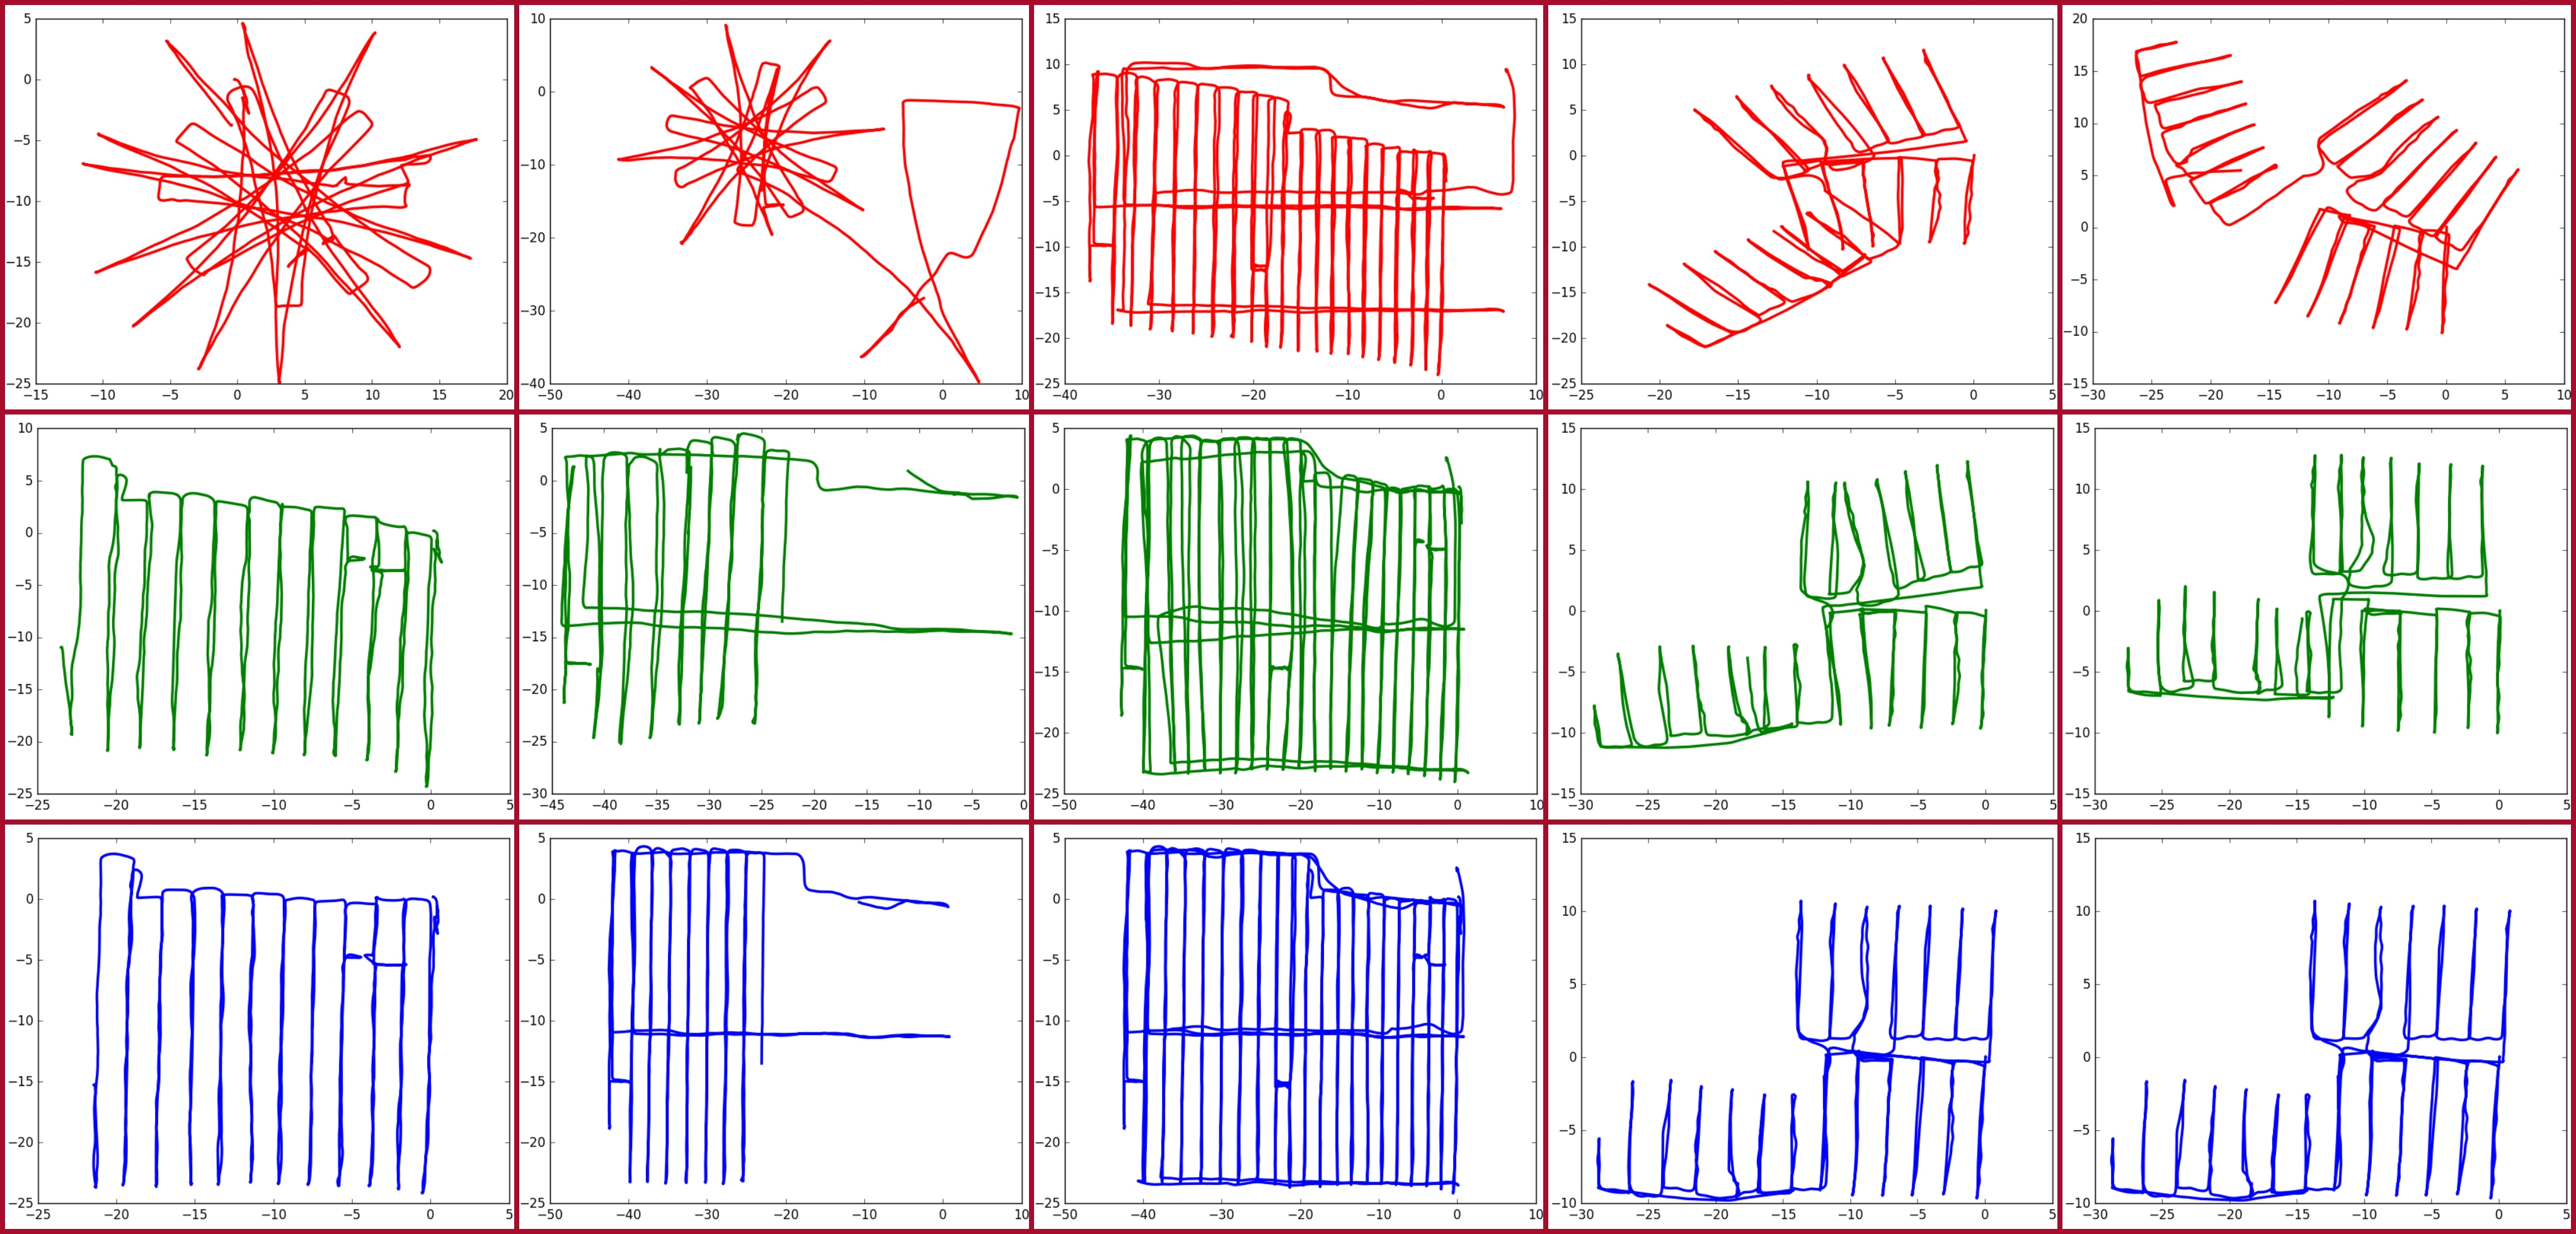
\includegraphics[width=300px,height=6cm]{pic/traj_recover.jpg}
		\caption{Top row shows unoptimized trajectories, middle row shows trajectories recovered using our pipeline and last row shows ground truth trajectories. Length in metres is shown along X and Y axes.}
		\label{fig:trajectory_recovery}
	\end{figure*}
	
	
	
	\section{Conclusion and Future Work}
	
	This paper shows how higher level abstractions of an indoor workspace such as real warehouses can be used to effectively improve lower level backend modules of localization and mapping. Specifically we show how higher and intermediate level abstractions in the form of Topological Graph and Manhattan Graph can recover from backend pose graph optimization failures. Further by constant information exchange between the various levels of map abstractions we improve quantitatively the ATE by more than 87.4\% starting from very distorted pose graphs. We further show the method is robust to failures in the higher level representations such, which occurs when the Deep CNN architecture wrongly classifies a topological construct or when the Siamese style classifier wrongly detects or fails to detect loops in the Manhattan graph. The results shown are on two different real warehouse scenes over an area of around $30m \times 50m$, filled with many repetitive topologies in the form of corridor areas and rackspaces. Future results are intended to be shown on a variety of indoor topologies and office spaces such as for example those found in the Gibson environment.
	
	\newpage
	\bibliographystyle{unsrt}
	\bibliography{citations}
	
\end{document}
